\documentclass[14pt,a4paper,report]{report}
\usepackage[a4paper, mag=1000, left=2.5cm, right=1cm, top=2cm, bottom=2cm, headsep=0.7cm, footskip=1cm]{geometry}
\usepackage[utf8]{inputenc}
\usepackage[english,russian]{babel}
\usepackage{indentfirst}
\usepackage[dvipsnames]{xcolor}
\usepackage[colorlinks]{hyperref}
\usepackage{listings} 
\usepackage{fancyhdr}
\usepackage{caption}
\usepackage{amsmath}
\usepackage{graphicx}
\usepackage{amsmath}
\usepackage{booktabs}
\usepackage{array}
\newcolumntype{P}[1]{>{\centering\arraybackslash}p{#1}}
\hypersetup{
	colorlinks = true,
	linkcolor  = black
}

\usepackage{titlesec}
\titleformat{\chapter}
{\Large\bfseries} % format
{}                % label
{0pt}             % sep
{\huge}           % before-code


\DeclareCaptionFont{white}{\color{white}} 

% Listing description
\usepackage{listings} 
\DeclareCaptionFormat{listing}{\colorbox{gray}{\parbox{\textwidth}{#1#2#3}}}
\captionsetup[lstlisting]{format=listing,labelfont=white,textfont=white}
\lstset{ 
	% Listing settings
	inputencoding = utf8,			
	extendedchars = \true, 
	keepspaces = true, 			  	 % Поддержка кириллицы и пробелов в комментариях
	language = Prolog,            	 	 % Язык программирования (для подсветки)
	basicstyle = \small\sffamily, 	 % Размер и начертание шрифта для подсветки кода
	numbers = left,               	 % Где поставить нумерацию строк (слева\справа)
	numberstyle = \tiny,          	 % Размер шрифта для номеров строк
	stepnumber = 1,               	 % Размер шага между двумя номерами строк
	numbersep = 5pt,              	 % Как далеко отстоят номера строк от подсвечиваемого кода
	backgroundcolor = \color{white}, % Цвет фона подсветки - используем \usepackage{color}
	showspaces = false,           	 % Показывать или нет пробелы специальными отступами
	showstringspaces = false,    	 % Показывать или нет пробелы в строках
	showtabs = false,           	 % Показывать или нет табуляцию в строках
	frame = single,              	 % Рисовать рамку вокруг кода
	tabsize = 2,                  	 % Размер табуляции по умолчанию равен 2 пробелам
	captionpos = t,             	 % Позиция заголовка вверху [t] или внизу [b] 
	breaklines = true,           	 % Автоматически переносить строки (да\нет)
	breakatwhitespace = false,   	 % Переносить строки только если есть пробел
	escapeinside = {\%*}{*)}      	 % Если нужно добавить комментарии в коде
}

\begin{document}

\def\contentsname{Содержание}

% Titlepage
\begin{titlepage}
	\begin{center}
		\textsc{Санкт-Петербургский Политехнический 
			Университет Петра Великого\\[5mm]
			Кафедра компьютерных систем и программных технологий}
		
		\vfill
		
		\textbf{Отчёт по лабораторной работе №4\\[3mm]
			Курс: «Язык искусственного интеллекта PROLOG»\\[41mm]
		}
	\end{center}
	
	\hfill
	\begin{minipage}{.4\textwidth}
		Выполнил студент:\\[2mm] 
		Бояркин Н.С.\\
		Группа: 13541/3\\[5mm]
		
		Проверил:\\[2mm] 
		Сазанов А.М.
	\end{minipage}
	\vfill
	\begin{center}
		Санкт-Петербург\\ \the\year\ г.
	\end{center}
\end{titlepage}

% Contents
\tableofcontents
\clearpage

\chapter{Лабораторная работа №4}

\section{Цель работы}

Ознакомиться с языком PROLOG и средой разработки Visual Prolog.

\section{Программа работы}

\begin{enumerate}
	\item Получите начальное представление о синтаксисе и семантике базовых конструкций языка PROLOG, ознакомившись с разделами 1-5 методического пособия [1]
	\item Создайте проект в оболочке Visual Prolog 7.3., как это показано в примере [2]
	\item Удалить проект, созданный в предыдущем пункте и запустить демонстрационный проект family1 в
	оболочке Visual Prolog 7.3.
	\item Постройте генеалогическое дерево для данного примера на основе результатов выполнения программы и исходного кода программы.
	\item Построить описание онтологии из данного примера на естественном языке. 
	\item Построить концептуальную карту (семантическую сеть), описывающую данный пример.
	\item Создать проекты 1-21 для каждого из примеров в пособии из п.1 и привести листинги результатов работы каждой из программ в ответ на запросы пользователя. 
	\item Выполнить индивидуальное задание для варианта 9 [3]
	\item Изучить 1-2 лабы по методичке [1] Согласно своему варианту решить задачу с помощью PROLOG.
	\item В выводах отразить следующее:
	\begin{itemize}
		\item В чем Плюсы и минусы языка Prolog?
		\item Какие еще языки используются для разработки ИИ, приведите примеры (НЕ МЕНЕЕ 2-х) проектов, языков и краткое описание проектов. (Альтернативы PROLOG)
		\item Решаема ли проблема комбинаторного взрыва, пути решения?
		\item Корректно ли по-вашему в принципе разработка языка ИИ? Что он должен из себя представлять?
		\item Можно ли разработать ИИ не понимая, как он работает, должны ли мы понимать, как он работает, думает, рассуждает?
	\end{itemize}
\end{enumerate}


\clearpage

\section{Ход работы}

\subsection{Запустите демонстрационный проект family1}

\begin{figure}[h!]
	\centering
	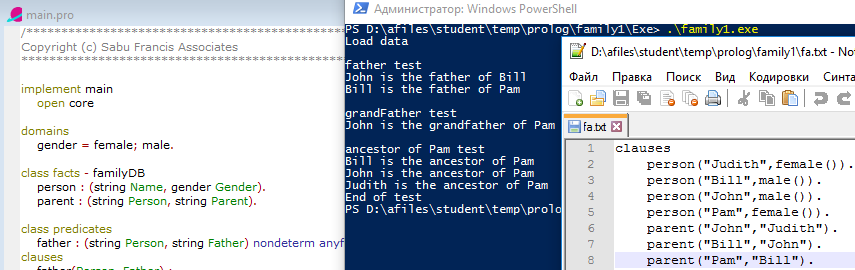
\includegraphics[scale = 0.75]{images/1.png}
	\caption{Запуск демонстрационного проекта}
\end{figure}

\subsection{Постройте генеалогическое дерево для данного примера на основе результатов выполнения программы и исходного кода программы}

\begin{figure}[h!]
	\centering
	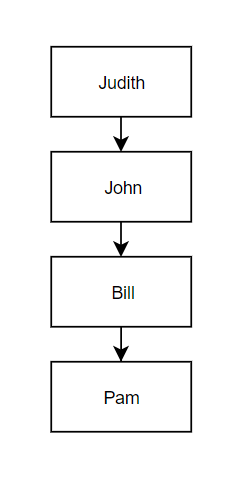
\includegraphics[scale = 0.65]{images/2.png}
	\caption{Генеалогическое дерево для конкретного примера}
\end{figure}

\subsection{Построить описание онтологии из данного примера на естественном языке}

Программа определяет степень родства между людьми. Входными данными для программы являются:

\begin{itemize}
	\item Имя и пол человека.
	\item Родительские связи.
\end{itemize}

На основании этих данных программа определяет:

\begin{itemize}
	\item Если человек является родителем и мужчиной, то он -- отец.
	\item Если человек является родителем другого родителя и мужчиной, то он -- дедушка.
	\item Если человек связан цепочкой родительских связей с другим человеком, то они -- родственники.
\end{itemize}

\subsection{Построить концептуальную карту (семантическую сеть), описывающую данный пример}

\begin{figure}[h!]
	\centering
	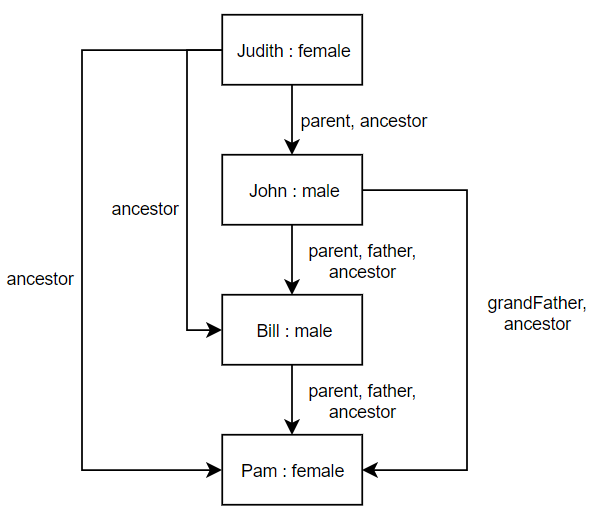
\includegraphics[scale = 0.65]{images/3.png}
	\caption{Концептуальная карта, описывающая данный пример}
\end{figure}

\subsection{Создать проекты 1-21 для каждого из примеров в пособии привести листинги результатов работы каждой из программ в ответ на запросы пользователя}

\subsubsection{Задание 1}

В программе выводятся все данные предиката situ. Кроме того, определены два правила, которые позволяют отнести города из России и Польши к городам Европы. 

\lstinputlisting{listings/1.pro}

\begin{figure}[h!]
	\centering
	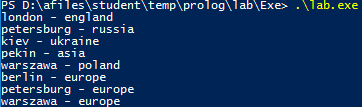
\includegraphics[scale = 1.0]{images/d1.png}
	\caption{Результаты выполнения задания}
\end{figure}

\subsubsection{Задание 2}

Составные объекты позволяют описывать иерархические структуры, в которых описание одного предиката включает в себя описание других предикатов. Данная программа иллюстрирует использование составных объектов:

\lstinputlisting{listings/2.pro}

\begin{figure}[h!]
	\centering
	
\includegraphics[scale = 1.0]{images/d2.png}
	\caption{Результаты выполнения задания}
\end{figure}

\subsubsection{Задание 3}

Программа описывает задачу о семейных отношениях. Имеются исходные данные об отцовстве: 

\begin{enumerate}
	\item Иван – отец Игоря.
	\item Иван – отец Сидора.
	\item Сидор – отец Лизы.
\end{enumerate}

Требуется определить, есть ли братья у Игоря. 


\lstinputlisting{listings/3.pro}

\begin{figure}[h!]
	\centering
	
\includegraphics[scale = 1.0]{images/d3.png}
	\caption{Результаты выполнения задания}
\end{figure}

\subsubsection{Задание 4}

Помимо встроенных функций для арифметических выражений можно использовать собственные предикаты. В данной программе осуществляется поиск суммы целых чисел, суммы вещественных чисел и максимума из двух вещественных чисел.

\lstinputlisting{listings/4.pro}

\begin{figure}[h!]
	\centering
	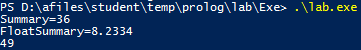
\includegraphics[scale = 1.0]{images/d4.png}
	\caption{Результаты выполнения задания}
\end{figure}

\subsubsection{Задание 5}

Программа находит страну, территория которой больше 1000000. Для использования анонимных переменных используется символ \_.

\lstinputlisting{listings/5.pro}

\begin{figure}[h!]
	\centering
	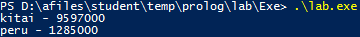
\includegraphics[scale = 1.0]{images/d5.png}
	\caption{Результаты выполнения задания}
\end{figure}

\subsubsection{Задание 6}

Используем собственный предикат hello() вместо стандартного run().

\lstinputlisting{listings/6.cl}

\lstinputlisting{listings/6.pro}

\begin{figure}[h!]
	\centering
	
\includegraphics[scale = 1.0]{images/d6.png}
	\caption{Результаты выполнения задания}
\end{figure}

\subsubsection{Задание 7}

В ПРОЛОГе реализован механизм поиска с возвратом (backtracking), при котором система пытается отыскать все возможные решения задачи. Механизм вывода программы запоминает те точки процесса унификации, в которых не были использованы все альтернативные решения, а затем возвращается в эти точки и ищет решение по иному пути.

Для реализации данного механизма без взаимодействия с пользователем используется предикат fail. 

\lstinputlisting{listings/7.cl}

\lstinputlisting{listings/7.pro}

\begin{figure}[h!]
	\centering
	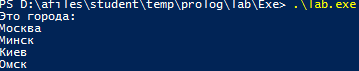
\includegraphics[scale = 1.0]{images/d7.png}
	\caption{Результаты выполнения задания}
\end{figure}

\subsubsection{Задание 8}

Программа демонстрирует работу предиката cut. При нахождении хотя бы одного соответствия целям дальнейшие поиски прекращаются. В данном случае будут выведены имена всех мальчиков, девочки будут отброшены. 

\lstinputlisting{listings/8.cl}

\lstinputlisting{listings/8.pro}

\begin{figure}[h!]
	\centering
	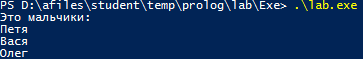
\includegraphics[scale = 1.0]{images/d8.png}
	\caption{Результаты выполнения задания}
\end{figure}

\subsubsection{Задание 9}

В программе осуществляется поиск машины светлого цвета дешевле 25000. Программа не найдет ни одного решения, поскольку после дорогих зеленых «жигулей» поиск заканчивается, и более дешевые «ауди» не будут найдены.

\lstinputlisting{listings/9.pro}

\begin{figure}[h!]
	\centering
	
\includegraphics[scale = 1.0]{images/d9.png}
	\caption{Результаты выполнения задания}
\end{figure}

\subsubsection{Задание 10}

В программе демонстрируется применение рекурсии. Будут напечатаны цифры от 1 до 9. В разделе clauses даны два описания предиката write\_number. Если в процессе решения первое описание не успешно, то используется второе описание.

\lstinputlisting{listings/10.pro}

\begin{figure}[h!]
	\centering
	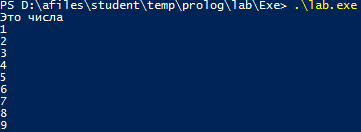
\includegraphics[scale = 1.0]{images/d10.png}
	\caption{Результаты выполнения задания}
\end{figure}

\subsubsection{Задание 11}

Данная программа печатает сумму всех цифр введенного числа. Использование предиката ! в описании нерекурсивного правила позволяет избежать здесь переполнения стека.

\lstinputlisting{listings/11.pro}

\begin{figure}[h!]
	\centering
	
\includegraphics[scale = 1.0]{images/d11.png}
	\caption{Результаты выполнения задания}
\end{figure}

\subsubsection{Задание 12}

Данная программа решает задачу «Ханойская башня». Требуется переместить диски с первого на третий стержень за некоторую последовательность ходов, каждый из которых заключается в перекладывания верхнего диска с одного из стержней на другой стержень. При этом больший диск никогда нельзя ставить на меньший диск.

В результате работы программы получено описание действий, необходимых для решения данной задачи.

\lstinputlisting{listings/12.pro}

\begin{figure}[h!]
	\centering
	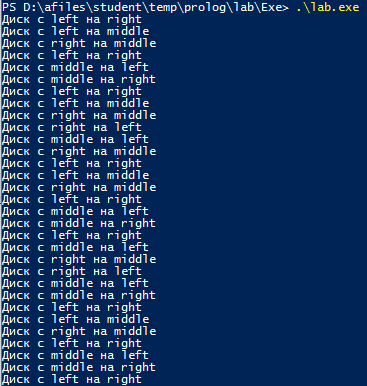
\includegraphics[scale = 1.0]{images/d12.png}
	\caption{Результаты выполнения задания}
\end{figure}

\subsubsection{Задание 13}

В данной программе используются списки. С их помощью описываются породы собак. Операция разделения списка на голову и хвост обозначается с помощью вертикальной черты: [Head|Tail]. С помощью этой операции можно реализовывать рекурсивную обработку списка и вывести элементы списка построчно.

\lstinputlisting{listings/13.pro}

\begin{figure}[h!]
	\centering
	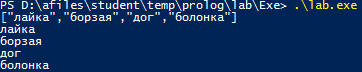
\includegraphics[scale = 1.0]{images/d13.png}
	\caption{Результаты выполнения задания}
\end{figure}

\subsubsection{Задание 14}

Первое правило описывает ситуацию, когда искомый элемент Х совпадает с головой списка. Второе правило используется при неуспехе первого правила и описывает новый вызов первого правила, но уже с усеченным списком, в котором нет первого элемента и т.д. Если в списке нет элементов (пустой список), то второе правило оказывается неуспешным.

Программа не напечатает Yes, поскольку болонки нет в списке собак.


\lstinputlisting{listings/14.pro}

\begin{figure}[h!]
	\centering
	
\includegraphics[scale = 1.0]{images/d14.png}
	\caption{Результаты выполнения задания}
\end{figure}

\subsubsection{Задание 15}

В данном примере производится подсчет суммы всех элементов списка. 

\lstinputlisting{listings/15.pro}

\begin{figure}[h!]
	\centering
	
\includegraphics[scale = 1.0]{images/d15.png}
	\caption{Результаты выполнения задания}
\end{figure}

\subsubsection{Задание 16}

Данный пример показывает, как используются списки и механизм рекурсии при решении известной задачи о мужике, волке, козе и капусте.

\lstinputlisting{listings/16.pro}

\begin{figure}[h!]
	\centering
	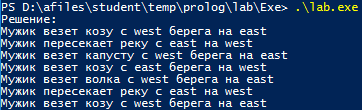
\includegraphics[scale = 1.0]{images/d16.png}
	\caption{Результаты выполнения задания}
\end{figure}

\subsubsection{Задание 17}

В данной программе решается следующая логическая задача:

«В велосипедных гонках три первых места заняли Алеша, Петя и Коля. Какое место занял каждый из них, если Петя занял не второе и не третье место, а Коля – не третье?»

\lstinputlisting{listings/17.pro}

\begin{figure}[h!]
	\centering
	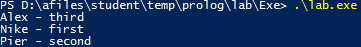
\includegraphics[scale = 1.0]{images/d17.png}
	\caption{Результаты выполнения задания}
\end{figure}

\subsubsection{Задание 18}

В данной программе решается следующая логическая задача:

«Пятеро студентов едут на велосипедах. Их зовут Сергей, Борис, Леонид, Григорий и Виктор. Велосипеды сделаны в пяти городах: Риге, Пензе, Львове, Харькове и Москве. Каждый из студентов родился в одном из этих городов, но ни один из студентов не едет на велосипеде, сделанном на его родине. Сергей едет на велосипеде, сделанном в Риге. Борис родом из Риги, у него велосипед из Пензы. У Виктора велосипед из Москвы. У Григория велосипед из Харькова. Виктор родом из Львова. Уроженец Пензы едет на велосипеде, сделанном на родине Леонида. Кто из студентов родом из Москвы?»

\lstinputlisting{listings/18.pro}

\begin{figure}[h!]
	\centering
	
\includegraphics[scale = 1.0]{images/d18.png}
	\caption{Результаты выполнения задания}
\end{figure}

\subsubsection{Задание 19}

В данной программе решается следующая логическая задача:

«Пять студентов должны посещать лекции всю неделю, но по определенным ими установленным правилам, а именно:
1. Если пришли Андрей и Дмитрий, то Бориса быть не должно, но если Дмитрий не пришел, то Борис должен быть, а Виктор быть не должен.
2. Если Виктор пришел, то Андрея быть не должно и наоборот.
3. Если Дмитрий пришел, то Григория быть не должно.
4. Если Бориса нет, то Дмитрий должен быть, но если нет также и Виктора, а если Виктор есть, Дмитрия быть не должно, но должен быть Григорий.
5. Каждый день студенты должны приходить в разных сочетаниях.
Какие это сочетания?»

\lstinputlisting{listings/19.pro}

\begin{figure}[h!]
	\centering
	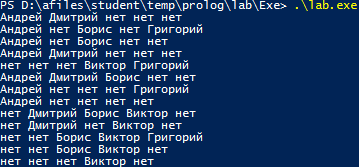
\includegraphics[scale = 1.0]{images/d19.png}
	\caption{Результаты выполнения задания}
\end{figure}

\subsubsection{Задание 20}

Факты, описанные в разделе clauses, можно рассматривать, как статическую базу данных (БД). Эти факты являются частью кода программы и не могут быть оперативно изменены. 

В данной программе осуществляется поиск человека, ростом выше 180 см. 

\lstinputlisting{listings/20.pro}

\begin{figure}[h!]
	\centering
	
\includegraphics[scale = 1.0]{images/d20.png}
	\caption{Результаты выполнения задания}
\end{figure}

\subsubsection{Задание 21}

Создадим простую экспертную систему, которая решает задачу определения вида экземпляра пойманной рыбы.

Программа реализует заданное дерево поиска решения. Ответы на заданные вопросы позволяют продвигаться по ветвям этого дерева к одному из вариантов решения.

\lstinputlisting{listings/21.pro}

\begin{figure}[h!]
	\centering
	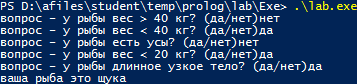
\includegraphics[scale = 1.0]{images/d21_1.png}
	\caption{Результаты выполнения задания}
\end{figure}

\begin{figure}[h!]
	\centering
	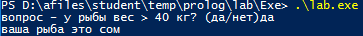
\includegraphics[scale = 1.0]{images/d21_2.png}
	\caption{Результаты выполнения задания}
\end{figure}

\begin{figure}[h!]
	\centering
	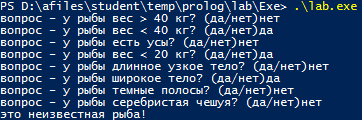
\includegraphics[scale = 1.0]{images/d21_3.png}
	\caption{Результаты выполнения задания}
\end{figure}

\subsection{Выполнить индивидуальное задание из пособия Буракова С.В.}

\textbf{Вариант 9}

Трое ребят вышли гулять с собакой, кошкой и хомячком. Известно, что Петя не любит кошек и живет в одном подъезде с хозяйкой хомячка. Лена дружит с Таней, гуляющей с кошкой. Определить, с каким животным гулял каждый из детей?

\lstinputlisting{listings/i1.pro}

Программа была выполнена по аналогии с задачей 17. Решение основывается на трех формализованных правилах:

\begin{enumerate}
	\item У Пети не кошка и не хомяк.
	\item У Тани кошка.
	\item У Лены оставшееся животное.
\end{enumerate}

Результат выполнения задания:

\begin{figure}[h!]
	\centering
	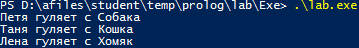
\includegraphics[scale = 1.0]{images/i1.png}
	\caption{Результаты выполнения индивидуального задания}
\end{figure}


\subsection{Выполнить индивидуальное задание из пособия Седана С.Н.}

Лабиринт представляет собой систему комнат, соединенных между собой переходами. В лабиринте имеется вход и выход, а также комната с золотым кладом. Кроме того, имеются комнаты, запрещенные для посещений: комната монстров и комната разбойников.

\begin{enumerate}
	\item Найди путь в лабиринте от входа до входа, не посещая дважды одной и той же комнаты;
	\item Найти путь с посещением золотой комнаты;
	\item Найти путь, избегающий запрещенных к посещению комнат.
\end{enumerate}

\lstinputlisting{listings/i2.pro}

В данном алгоритме указываются связи между соседними комнатами, после чего подбираются различные варианты маршрутов, с помощью path. Кроме того, на path установлен фильтр, который выводит в консоль все варианты пути, удовлетворяющие фильтру. Таким образом выполняются условия с типами комнат.

Результат выполнения задания:

\begin{figure}[h!]
	\centering
	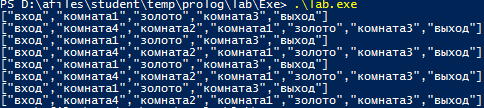
\includegraphics[scale = 1.0]{images/i2.png}
	\caption{Результаты выполнения индивидуального задания}
\end{figure}

Варианты правильные, однако, повторяются несколько раз. Этого можно избежать, если заменить writef внутри функции на возвращаемый список, который впоследствии будет отфильтрован на предмет одинаковых вариантов.


\section{Вывод}

В результате работы были изучены основные возможности языка Prolog, а также среды разработки Visual Prolog.

\subsubsection{Плюсы и минусы языка Prolog}

К плюсам языка Prolog относится тот факт, что это декларативный язык: описывается логическая модель предметной области (ПО) в терминах этой ПО, их свойства и отношения между ними, а не детали программной реализации. Таким образом, мы описываем «что» хотим получить, а не «как» мы хотим это получить. Это позволяет сильно уменьшить время разработки приложений и размеры исходного кода.

Из минусов этого языка можно выделить его узкую специализацию. Язык хорошо показывает себя в своей области применения, однако, для написания чего-то универсального и производительного он не годится.

\subsubsection{Аналоги языка Prolog}

Существует множество аналогов языка PROLOG, например:

\begin{itemize}
	\item Python -- язык, который содержит огромный набор научных библиотек, в том числе и для ИИ.
	\item CLIPS -- программная среда и язык для разработки экспертных систем.
	\item Planner -- функционально-логический язык программирования, схожий по своему синтаксису с LISP.
	\item Linden Scripting Language (или LSL) -- скриптовый язык программирования.
	\item LISP -- функциональный язык программирования.
\end{itemize}

\subsubsection{Проблема комбинаторного взрыва}

Проблема комбинаторного взрыва в общем случае не решена, однако, использование метода наискорейшего подъема помогает значительно ускорить поиск.

\subsubsection{Корректность разработки языка ИИ}

Идея разработки языка ИИ не только корректна, но и необходима. Кроме того, существующие языки в этой области должны быть или улучшены, или заменены более совершенными и удобными языками. Это позволит значительно ускорить создание полноценного ИИ. Разумеется, обязательным качеством такого языка должна являться декларативность.

\subsubsection{Понимание ИИ}

Понимание о идеальном ИИ должно быть поверхностным, на уровне основных высокоуровневых компонентов и ограничений. Все остальное нужно предоставить самому ИИ на самостоятельное обучение. Это также соответствует декларативной концепции -- мы должны знать что делает ИИ, но не должны знать как.

\section{Список литературы}

% \linebreak

\begin{flushleft}
	
[1] Середа С.Н. «Методичка по языку Prolog», Муромский университет. 2003г.\linebreak

[2] Основы Системы Visual Prolog [Электронный ресурс]. — URL: \href{http://wikiru.visual-prolog.com/index.php?title=\%D0\%9E\%D1\%81\%D0\%BD\%D0\%BE\%D0\%B2\%D1\%8B\_\%D0\%A1\%D0\%B8\%D1\%81\%D1\%82\%D0\%B5\%D0\%BC\%D1\%8B_Visual_Prolog}{http://wikiru.visual-prolog.com/index.php?title=\%D0\%9E\%D1\%81\%D0\%BD\%D0\%BE\%D0\%B2\%D1\%8B\_\%D0\%A1\%D0\%B8\%D1\%81\%D1\%82\%D0\%B5\%D0\%BC\%D1\%8B\_Visual\_Prolog} (дата обращения 27.10.2017). \linebreak
	
[3] ЯЗЫК ЛОГИЧЕСКОГО ПРОГРАММИРОВАНИЯ ПРОЛОГ, М.В. Бураков [Электронный ресурс]. — URL: \href{http://www.ict.edu.ru/ft/005578/byrakov.pdf}{http://www.ict.edu.ru/ft/005578/byrakov.pdf} (дата обращения 27.10.2017). \linebreak





\end{flushleft}
	


\end{document}